\section{Reactive approach}
\label{reactive-approach}
Due to the high variability of the input rate, the adaptation of SPS resources is necessary for performance sake. In this first proposal, denoted \rSPS{}, we use a reactive model to analyse the state of the operators to modify the number of active replicas of the operators in the DAG. Table \ref{tab:rsps-notations} summarises all parameters used in \rSPS{}.

\begin{table}[!ht]
\begin{tabular}{|c|l|}
    \hline
    \textit{\textbf{Parameter}}     & \textit{\textbf{Description}}             \\  \hline
    $O_i$			& operator $i$ \\
    $t$				& time interval number \\ 
    $td$			& time interval duration  \\
    $et_i(t)$		& average execution time of one event by $O_i$ during $t$ \\
    $et_i$		& average execution time of one event by $O_i$ according to the benchmark\\
    $q_i(t)$		& queue of events received and not processed by $O_i$ at the end of $t$ \\
    $\mu_i(t)$		& number of events processed by $O_i$ during $t$\\
    $r_i(t)$ 		& number of active replicas of $O_i$ during $t$ \\
    $U_i(t)$		& Utilization metric by $O_i$ during $t$ \\
    $E_i(t)$		& Execution Time metric by $O_i$ during $t$ \\
    $Q_i(t)$		& Queue metric by $O_i$ during $t$ \\
    $\delta_i(t)$	& State metric by $O_i$ during $t$ \\
    \hline
\end{tabular}
\caption{Parameters notation and their description in \rSPS{}.}
\label{tab:rsps-notations}
\end{table}


\subsection{Metrics}
An adaptive SPS should define metrics to characterize the state of the operators at runtime on a given scenario. Traditional metrics such as throughput, latency, and CPU are the most used in literature (see Section \ref{rw-auto-reactive}). In \rSPS{}, we propose to integrate the metrics denoted \textit{Utilization ($U$)}, \textit{Execution Time ($E$)}, \textit{Queue ($Q$)} and \textit{State} ($\delta$).

\textit{Utilization} metric  is defined by Equation \ref{eq:rsps-utilization}. The aim of the metric is to characterize the operator load: if its value is close to 1 (resp., 0), the operator is overloaded (resp., underloaded). Figure \ref{fig:prediction-replicas} shows an example composed of three independent operators ($O_1$, $O_2$, and $O_3$) that have different $U_i(t)$.

\begin{equation}
\label{eq:rsps-utilization}
        U_i(t) = \frac{\mu_i(t) \times et_i(t)}{r \times td}
\end{equation}

In Figure \ref{fig:rsps-metric-u}, the three operators have 2 replicas ($r_i=2$) and an average execution time of 200 milliseconds ($e_i=200~ms$). As the number of events processed is different during the time interval $t$ for each operator, their loads are different. $O_1$ has no idle time, so it is at maximum utilization, so the operator is overloaded. $O_2$ has a load level which is $50\%$ of the time idle in time period $t$. $O_3$ is almost underloaded.

\begin{figure}[!ht]
    \centering
    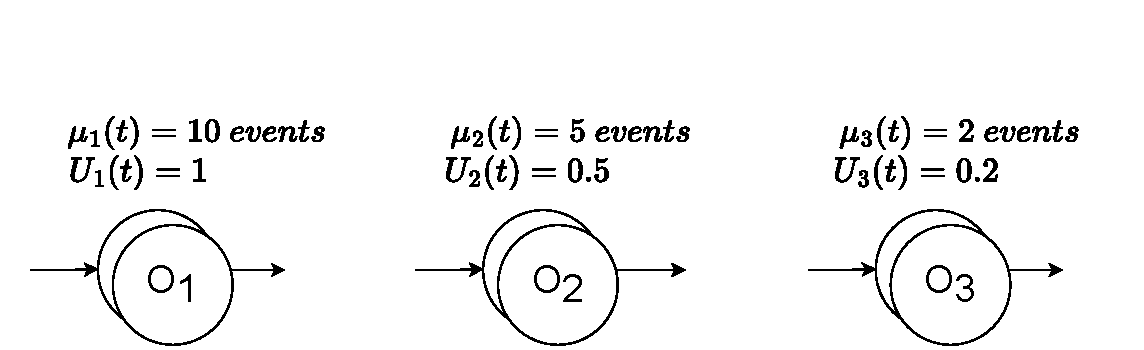
\includegraphics[width=0.8\textwidth]{figures/concepts/RA-SPS-Metric-U.pdf}
    \caption{Example of the \textit{Utilisation} metric.}
    \label{fig:rsps-metric-u}
\end{figure}


\textit{Execution Time} metric  is defined by Equation \ref{eq:rsps-latency}. The aim of the metric is to characterize execution degradation of operators: if the value of $et_i(t)$ is greater than $et_i$, the physical machines are overloaded. It is a QoS metric which allows to detect struggle operators. Therefore, the difference between $et_i(t)$ and $et_i$ is that the latter is the average execution time of one event processed by an operator $O_i$ without any extra load. The variable $et_i$ is considered as a baseline, and it is estimated by previously  benchmark execution.

\begin{equation}       
        E_i(t) = 1-\frac{et_i}{et_i(t)}
\label{eq:rsps-latency}
\end{equation}

In Figure \ref{fig:rsps-metric-e}, the three operators have an average execution time of 200 milliseconds ($et_i=100$). $O_1$ has a large extra load, possibly due to overutilisation of resources, so the execution time is much longer. Unlike $O_3$, which has no extra load, or $O_2$ which has less extra load.

\begin{figure}[!ht]
    \centering
    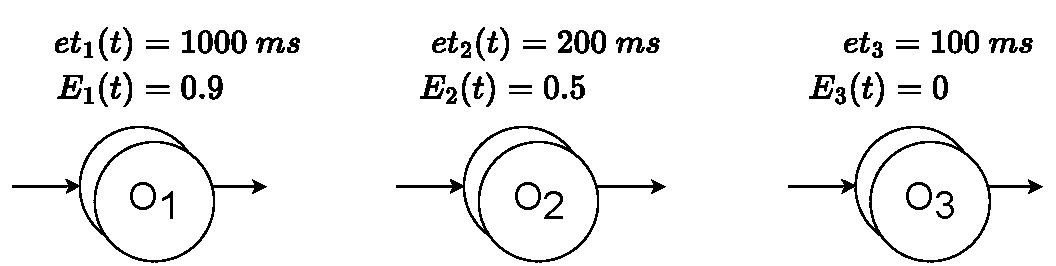
\includegraphics[width=0.8\textwidth]{figures/concepts/RA-SPS-Metric-E.pdf}
    \caption{Example of the \textit{Execution Time} metric.}
    \label{fig:rsps-metric-e}
\end{figure}

\textit{Queue} metric is defined by Equation \ref{eq:rsps-queue}. The aim of the metric is to analyze the impact of the input queue on the operator with respect to its current processing capacity. The $Q_i(t)$ tackles the input traffic behavior (traffic shape). Sudden peaks will increase the number of the events queued, $q_i(t)$ value, generating higher values of $Q_i(t)$. If $q_i(t)$ value is 0 or $Q_i(t)$ value is negative, its value is set to 0.

\begin{equation}
        Q_i(t) = 1-\frac{\mu_i(t)}{q_i(t).}
\label{eq:rsps-queue}
\end{equation}

In Figure \ref{fig:rsps-metric-q}, the three operators have 10 processed events ($\mu_i(t)=10~events$). In the case of $O_1$, it has a small tail, so its impact is minimal. Compared to $O_1$, $O_2$ has a larger number of queued events, which is reflected by the increase of metric value. Finally, $O_3$ has a considerable high $Q_{3}(t)$ value, due to the large number of queued events.

\begin{figure}[!ht]
    \centering
    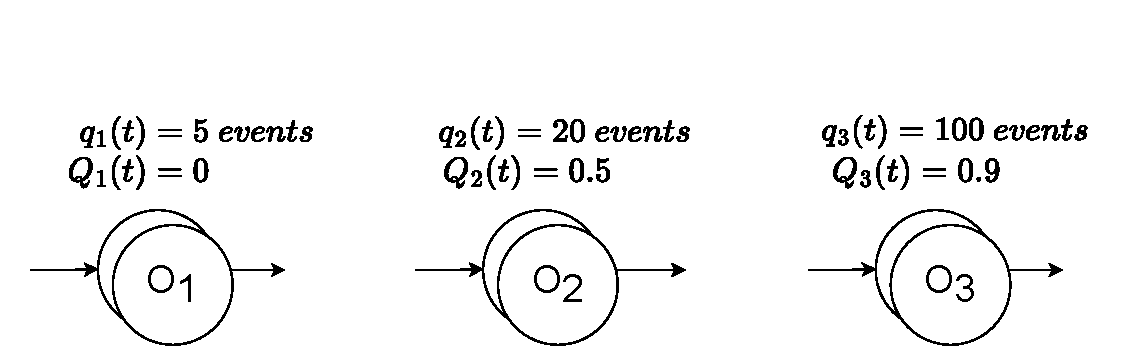
\includegraphics[width=0.8\textwidth]{figures/concepts/RA-SPS-Metric-Q.pdf}
    \caption{Example of the \textit{Queue} metric.}
    \label{fig:rsps-metric-q}
\end{figure}

To determine the overall state of an operator, the \textit{State} metric, denoted $\delta_i(t)$, is defined by Equation \ref{eq:rsps-delta}. It uses the previously defined metrics $U_i(t)$, $Q_i(t)$, and $E_i(t)$. By introducing weights ($\omega_U$, $\omega_Q$, and $\omega_E$), the impact of the 3 metrics can be balanced, allowing, therefore, the study of the relevance of each metric in different load scenarios.

\begin{equation}
    \delta_i(t) = U_i(t) \times \omega_U + Q_i(t) \times \omega_Q + E_i(t) \times \omega_E
    \label{eq:rsps-delta}
\end{equation}

The $\delta_i(t)$ value characterizes the overall state of an operator as shown in Figure \ref{fig:rsps-metric-state}. Following a threshold-based approach, two bounds are defined: the upper bound $\delta_{u}$ and the lower bound $\delta_{l}$. Considering these bounds, an operator can be in one of the three following states: \textit{overloaded}, \textit{stable}, or \textit{underloaded}. These states give information about an operator's \textit{effectiveness} and \textit{efficiency}. \textit{Effectiveness} is the capacity to fully process the input data, while \textit{efficiency} is the capacity to process data by taking advantage of the available resources. If an operator is \textit{overloaded}, it is not capable of processing all the input data, losing efficiency. On the other hand, if the operator is \textit{underloaded}, it processes the input data effectively but not efficiently. Finally, an operator whose state is \textit{stable} processes input data both efficiently and effectively.

\begin{figure}[!ht]
    \centering
    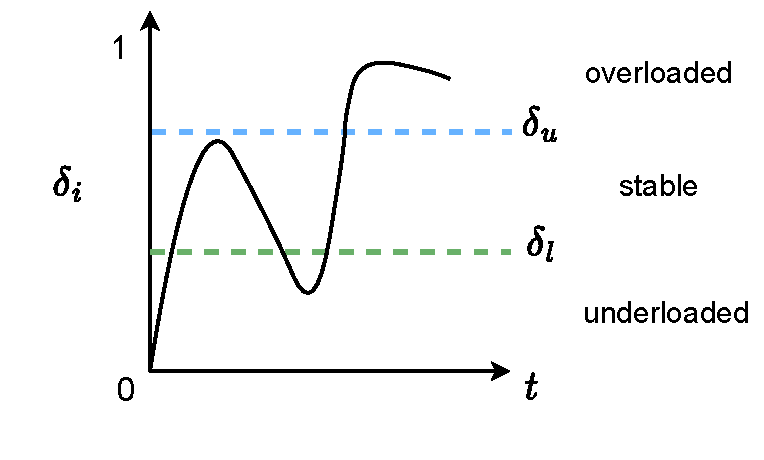
\includegraphics[width=0.5\textwidth]{figures/concepts/RA-SPS-Metric-Delta.pdf}
    \caption{Example of the evolution of the \textit{State} metric in the operator $O_i$.}
    \label{fig:rsps-metric-state}
\end{figure}

\subsection{MAPE implementation}
Monitoring, Analysis, Planning, and Execution compose the MAPE control loop. This model is exploited in most autonomic systems. By repeating these four steps, the system can detect issues by analysing data. If a problem is found, a strategy is developed and the executed to solve the issue. The MAPE control loop brings the system autonomic features such as self-configuration and self-optimization. Figure \ref{fig:rsps-mape} presents the
architecture of \rSPS{}:

\begin{figure}[!ht]
    \centering
    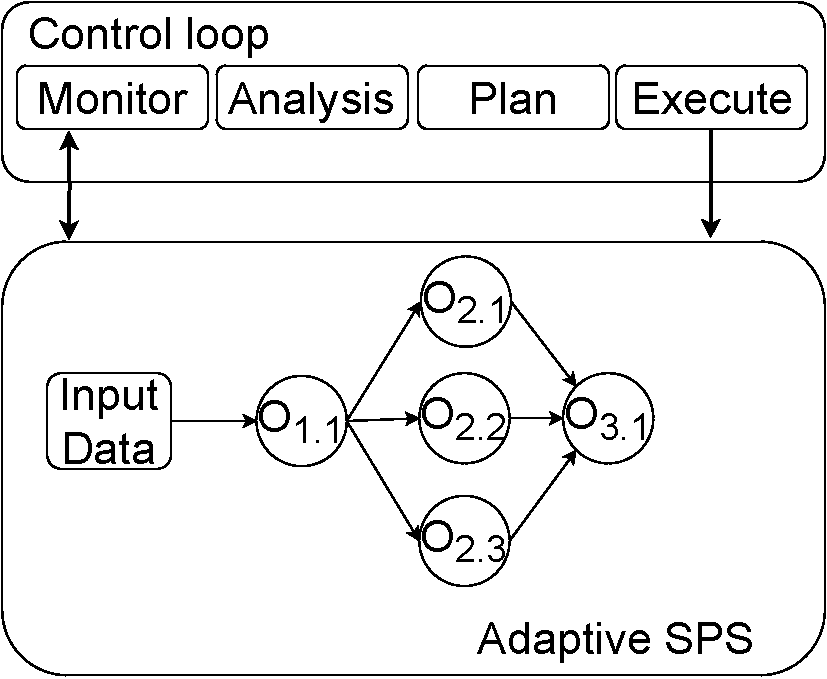
\includegraphics[width=0.45\textwidth]{figures/concepts/RA-SPS-Architecture.pdf}
    \caption{The architecture of \rSPS{}.}
    \label{fig:rsps-mape}
\end{figure}

In our system, the MAPE model integrates the before-mentioned components where each of the four MAPE modules performs the following tasks: 
\begin{enumerate} 
    \item \textit{Monitor}: module in charge of collecting statistics from the DAG. At a predefined time interval $t$, the monitor requests the values of $\mu_i(t)$, $et_i(t)$, and the number of queued events $q_i$.
    \item \textit{Analysis}: The module analyses the metrics of each operator and determines its status according to Equation \ref{eq:rsps-delta}.    
    \item \textit{Plan}: Based on the previous analysis, the \textit{Plan} module defines whether it is necessary or not to modify the system resource capacity. See Algorithm \ref{alg:rsps-planning} presented in Section \ref{rsps-planning}.
    \item \textit{Execute}: module in charge of carrying out the change in an operator's current number of replicas, if required by the \textit{Plan} module.
\end{enumerate}

\subsection{Planning}
\label{rsps-planning}

Algorithm \ref{alg:rsps-planning} that presents the algorithm executed by the \textit{Plan} module for the $O_i$ operator, deciding if the number of replicas of $O_i$ should be increased (or decreased) by $k$ or remain the same.
It uses a fixed value for $k$ for the \rSPS{} evaluation (see Section \ref{exp:params}). However, it is possible to dynamically modify this variable for the adaptation of the SPS.

Therefore, the aim of the algorithm is to modify the number of replicas of an operator $O_i$. If the operator is overloaded in line 3 ($\delta_i(t) > \delta_u$) or underloaded in line 7 ($\delta_i(t) < \delta_l$), the number of replicas should be increased or decreased respectively by $k$ replicas. Otherwise, if the operator state is stable, the number of replicas will not change. In order to ensure system stability, we define that an operator must remain in the same state by at least two consecutive time windows in line 2 ($\delta_i(t) = \delta_i(t-1)$) before carrying out any change in the number of replicas.

While the size of the pool of replicas is defined by the amount of cores, in case there is an overload of physical resources (VMs or nodes), it is necessary to limit the number of active replicas. For this, we determine a threshold $\delta_{E}$ for the metric $E_i(t)$, because the value of $E_i(t)$ indicates the degradation of the processing of the operator $O_i$. If $E_i(t)$ is greater than the threshold $\delta_{E}$ (line 4), the planning cannot increase the number of active replicas. In this way, we avoid an overload on the physical resources of the system and performance degradation of the SPS.

\begin{algorithm}[!ht]
 \caption{Adaptive planning algorithm according to the reactive approach for the operator $O_i$.}
 \begin{algorithmic}[1]
 	\REQUIRE Statistics Operator $O_i$ in time interval $t$.
 	\ENSURE Modifying the current number of active replicas of operator $O_i$.
	\STATE $\delta_i(t)$ $\gets$ calculateMultiMetric($U_i(t)$ , $Q_i(t)$ , $E_i(t)$)
	\IF {$\delta_i(t) = \delta_i(t-1)_i$}
		\IF {$\delta_i(t) > \delta_{u}$}
			\IF {$E_i(t) > \delta_{E}$}
				\STATE Add $k$ active replicas for $O_i$
			\ENDIF 
		\ELSIF {$\delta_i < \delta_{l}$}
			\STATE Remove $k$ active replicas for $O_i$
		\ENDIF
	\ENDIF
\end{algorithmic}
\label{alg:rsps-planning}
\end{algorithm}